\section{Proprietäre Systeme}

\begin{frame}{CUL}
	\begin{columns}
		\begin{column}[c]{0.45\textwidth}
			\begin{block}{CUL}
			\begin{itemize}
			\item 	RF-Device in Form eines USB-Dongles \linebreak
					(externe Antenne)
			\item 	Open-Source-Software (culfw) unterstützt verschiedene Protokolle
			\item 	verschiedene Modi: Slow-RF und \enquote{AskSin}
			\item 	\alert{kein Mischbetrieb zwischen Slow-RF und AskSin}
			\end{itemize}
			\end{block}
		\end{column}
		\begin{column}[c]{0.45\textwidth}
			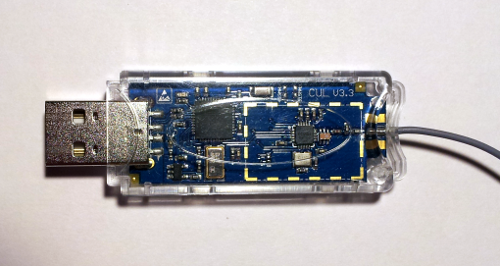
\includegraphics[width=\linewidth]{Cul}
			\begin{block}{Protokolle}
				\begin{itemize}
				\item 	Slow-RF: \linebreak
						\textbf{FS20}, \textbf{FHT}, EM, \linebreak
						S300, HMS, \ldots
				\item 	AskSin: \linebreak
						\textbf{HomeMatic}
				\end{itemize}
			\end{block}
		\end{column}
	\end{columns}
\end{frame}

\subsection{FS20}

\begin{frame}{FS20}

\begin{block}{Wirtschaftliche Lage}
\begin{itemize}
\item 	Verfügbarkeit: eine Vielzahl an Hardware
\item 	Preisniveau: moderat
\end{itemize}
\end{block}

\begin{block}{Eigenschaften}
\begin{itemize}
\item 	Nachrichtenaustausch: unverschlüsselt, keine Bestätigung
\item 	Pairing: simpel \eg{(Pairing-Modus aktivieren, Setzen von IDs via Kommandos)}
\item 	Unterscheidung zwischen Hauscode und Devicecode
\item 	Kommunikation: CUL \eg{(Firmware culfw)}
\end{itemize}
\end{block}
\end{frame}

\begin{frame}{FS20}{Stand}

\begin{block}<+->{Funksteckdose (FS20 ST-2)}
\begin{itemize}
\item 	Aktorknoten
\item 	reine FS20-Komponente
\item 	schaltbar \eg{(aus Python heraus)}
\end{itemize}
\end{block}

\begin{block}<+->{Funk-Tür-Fensterkontakt (FHT 80TF-2)}
\begin{itemize}
\item 	Sensorknoten
\item 	keine reine FS20-Komponente (FHT-Protokoll)
\item 	CUL unterstützt nicht nur FS20,
		sondern auch FHT und viele weitere Protokolle
\item 	Nachrichten werden empfangen und können ausgewertet werden
\end{itemize}
\end{block}
\uncover<3->{\alert{$\Rightarrow$ für den Prototypen ausreichend}}
\end{frame}

\subsection{HomeMatic}

\begin{frame}{HomeMatic}{Vergleich zu FS20}
		\centering
	\begin{tabular}{lcc}
	\toprule
	           & \textit{FS20} & \textit{HomeMatic} \tabularnewline
	\midrule
	Preisniveau & moderat & teuer \tabularnewline
	Gerätevielfalt & groß & klein \tabularnewline
	Frequenzband & \multicolumn{2}{c}{868 MHz} \tabularnewline
	Authentifizierung & keine & AES \tabularnewline
	Übertragung & unverschlüsselt & XOR-verschlüsselt  \tabularnewline
	Empfangsbestätigung & nein & ja  \tabularnewline
	\multirow{2}{*}{Sonstiges} & \multirow{2}{*}{Funktionsgruppen} & drahtgebundene \tabularnewline
	                           &                                   & Komponenten\tabularnewline
	\bottomrule
	\end{tabular}
\end{frame}

\begin{frame}{HomeMatic}{Stand / Vorgehen}
\begin{block}{Vorgehen}
\begin{itemize}
\item 	Analyse des Quellcodes von FHEM zum Verständnis des HomeMatic
		zugrunde liegenden Protokolls
\item 	Validierung des Protokolls durch Mitschnitte per CUL
\end{itemize}
\end{block}

\begin{block}{Stand}
\begin{itemize}
\item 	Funk-Zwischenstecker-Schaltaktor 1fach: Empfang und Auswertung des Paketes erfolgriech
\item 	Funk-Handsender 4 Tasten: Empfang und Auswertung des Paketes erfolgriech
\item 	Steuern eines Aktors ist noch offen
\end{itemize}
\end{block}
\end{frame}

